\begin{slide}{Fitting in $R$- or $k$-space:  What do we model?}

  \begin{cenpage}{135mm}
  The $\chi^2$ definition didn't say anything about what our data
  $\chi_i^{\rm measured}$ actually is \ldots

  \onslide+<2->
  \vmm  We usually fit in $R$-space, so that  we can select which
  ``shells'' to ignore:

  \vmm \vmm

  \begin{columns}
    \begin{column}{65mm}
      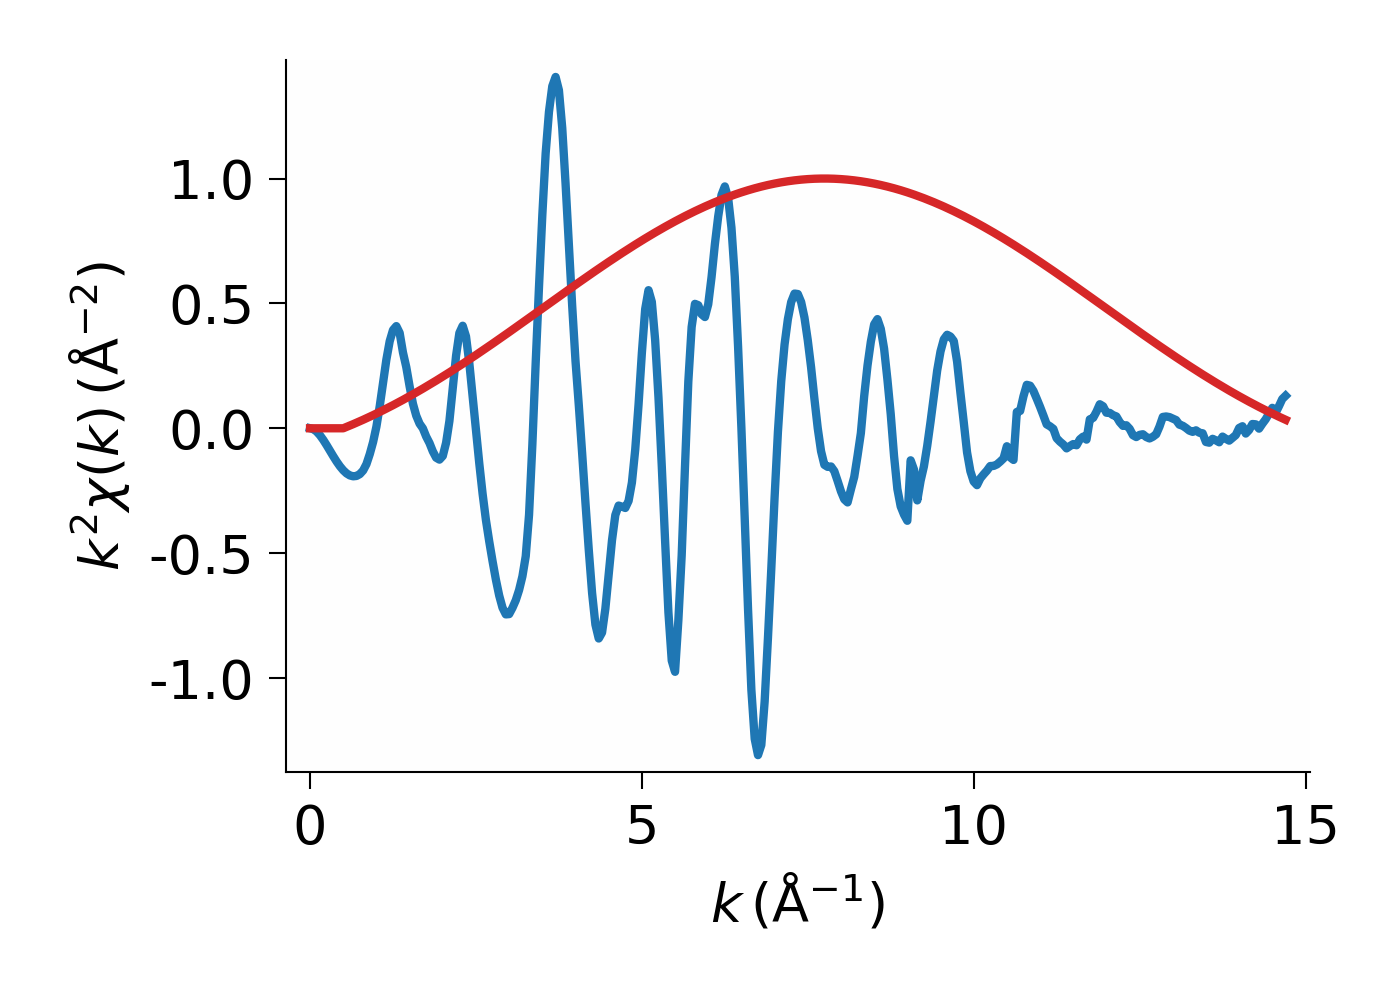
\includegraphics[width=60mm]{figs/experiment/chikw_win}
    \end{column}
    \begin{column}{65mm}
      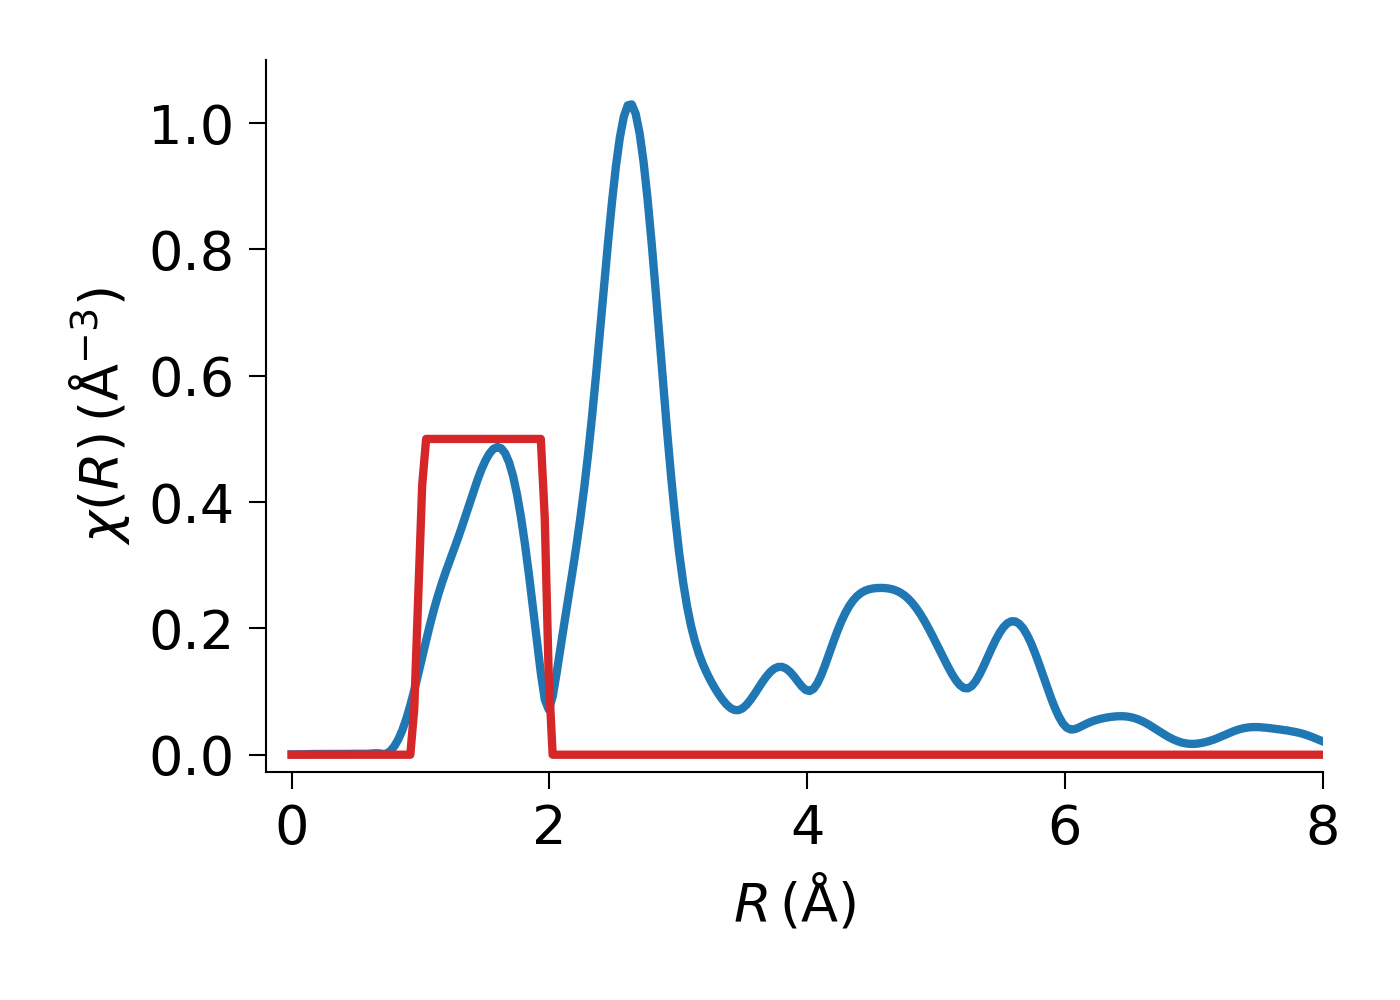
\includegraphics[width=60mm]{figs/experiment/chir_win}
    \end{column}
  \end{columns}

  \onslide+<3->
  Fitting $\chi(R)$ (both real and imaginary parts!) gives more
  meaningful fit statistics -- we know that we're not fitting all the
  spectral features.

  \vmm
  {\RedEmph{Plus:}}    We can have $\chi_i^{\rm measured}$  extend over
    {\Red{multiple data sets}}, {\Red{multiple $k$-weightings}},  etc.

    \vmm
  as long as we generate the corresponding {\Red{$\chi_i^{\rm model}(x)$}} to
  match these data.

  \vfill
  \end{cenpage}
\end{slide}
